% !TeX program = lualatex
% Copyright (C) 2026 Amer Amikhteh. LPPL 1.3c or later.
% Presentation helpers adapted from the BabelBidi manual, which adapts
% Babel's user guide (babel.dtx, version 26.14, 2026-10-15).
% Copyright (C) 2012-2026 Javier Bezos and Johannes L. Braams;
% Copyright (C) 1989-2012 Johannes L. Braams and individual authors.
% Changes: compact title panel, two-page companion text, minted examples.
% Compile from the distribution root (twice; requires minted/latexminted):
%   xelatex -shell-escape -halt-on-error -output-directory=doc doc/amikhteh-logo.tex
\documentclass[a4paper]{ltxdoc}
% Also find the source-tree copy when running from doc/.
\makeatletter
\providecommand\input@path{}
\g@addto@macro\input@path{{../}}
\makeatother
\usepackage{fontspec}
\usepackage[manual]{amikhteh-logo}
\usepackage{pkgmeta}
\usepackage{minted}
\usepackage{etoolbox}
\usepackage{needspace}
\usepackage{hyperref}

% The manual's English body fonts, with the same fallbacks and scales.
\IfFontExistsTF{Noto Serif}
{\setmainfont[Scale=.88]{Noto Serif}}{\setmainfont{Latin Modern Roman}}
\IfFontExistsTF{Noto Sans}
{\setsansfont[Scale=.88]{Noto Sans}}{\setsansfont{Latin Modern Sans}}
\IfFontExistsTF{DejaVu Sans Mono}
{\setmonofont[Scale=.86,FakeStretch=.97,AutoFakeSlant=.2]{DejaVu Sans Mono}}
{\setmonofont[Scale=MatchLowercase]{Latin Modern Mono}}

\definecolor{thered}{rgb}{0.65,0.04,0.07}
\definecolor{thegreyed}{gray}{0.6}
\definecolor{shadecolor}{rgb}{0.97,0.97,0.94}
\definecolor{bbCoverInk}{HTML}{283F46}
\definecolor{bbCoverCream}{HTML}{EBDDB9}
\definecolor{bbCoverRose}{HTML}{DDBBAA}

% Match the ltxdoc body geometry and documentation helpers in BabelBidi.
\addtolength{\oddsidemargin}{-2em}
\addtolength{\evensidemargin}{-2em}
\addtolength{\textwidth}{25.5pt}
\addtolength{\textheight}{3.5cm}
\addtolength{\topmargin}{-2cm}
\setlength{\emergencystretch}{2em}
\frenchspacing
\raggedright
\setlength{\parindent}{.8em}
\makeatletter
\def\Describe#1#2{%
    \par\vskip 1.7ex plus .7ex minus .2ex
    \noindent\hspace*{-1.7cm}%
    {\color{thegreyed}\normalsize\ttfamily
        \underline{\strut{\color{thered}\string#1}\color{black}#2}}%
    \par\nobreak\vskip 1.1ex plus .2ex\relax
}
\makeatother
% Match BabelBidi's minted style. Trim blank edge lines and keep the
% surrounding skips fixed, rather than compensating with negative space.
\usemintedstyle{friendly}
\setminted{
    fontsize=\small,
    breaklines=true,
    autogobble=true,
    bgcolor=shadecolor,
    bgcolorpadding=1.5mm,
    frame=single,
    framerule=.4pt,
    framesep=1.5mm,
    rulecolor=\color{black!45},
    baselinestretch=1
}
\hypersetup{
    colorlinks=true,linkcolor=thered,urlcolor=blue,citecolor=thered,
    pdfdisplaydoctitle=true,bookmarksnumbered=true,
    pdftitle={The amikhteh-logo Package -- Companion Guide},
    pdfauthor={Amer Amikhteh},
    pdfsubject={Shared author identity for the BabelBidi package family}
}
\AmikhtehLogoFooterSetup{size=9mm,footskip=14mm}
\pagestyle{amikhteh-logo}

\begin{document}
    % A compact version of the manual's cover palette, not a separate cover.
    \noindent
    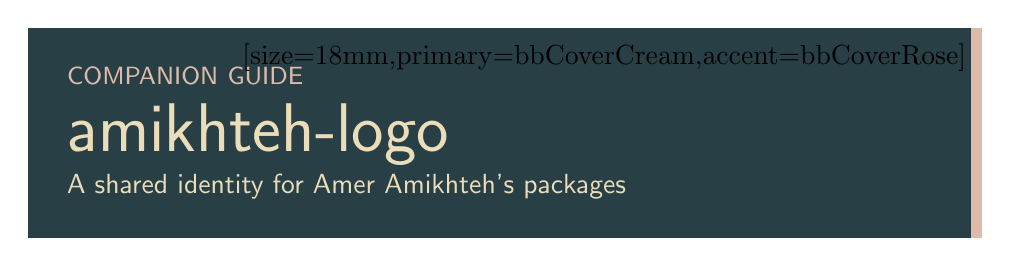
\begin{tikzpicture}
        \node[fill=bbCoverInk,inner sep=5mm,outer sep=0pt,
        text width=\dimexpr\linewidth-10mm\relax,align=left] (panel) {%
            {\sffamily\small\color{bbCoverRose}COMPANION GUIDE}\par\medskip
            {\sffamily\fontsize{29}{33}\selectfont\color{bbCoverCream}amikhteh-logo}\par\smallskip
            {\sffamily\color{bbCoverCream}A shared identity for Amer Amikhteh's packages}%
        };
        \fill[bbCoverRose] ([xshift=-1.5mm]panel.south east)
        rectangle (panel.north east);
        \node[anchor=north east,inner sep=2mm] at (panel.north east)
        {\AmikhtehLogo[size=18mm,primary=bbCoverCream,accent=bbCoverRose]};
    \end{tikzpicture}\par\smallskip
    \noindent Version \pkgmeta[version]{amikhteh-logo}\quad---\quad
    \pkgmeta[date]{amikhteh-logo}\hfill Amer Amikhteh

    \section{Purpose and loading}
    \textsf{amikhteh-logo} holds the author's identity mark shared by
    BabelBidi, UniPersian and future packages. It is a BabelBidi companion,
    not a separate release or a general-purpose logo collection. Install
    \texttt{amikhteh-logo.sty} with BabelBidi's public \TeX\ files; no copies
    belong in individual documentation directories. The author's packages
    are listed at \url{https://ctan.org/author/amikhteh}.
    \begin{minted}{latex}
        \usepackage{amikhteh-logo}
    \end{minted}
    It is not loaded by \texttt{babelbidi.sty} and does not itself load
    BabelBidi, select languages or fonts, or change paragraph direction or
    page layout. It needs TikZ and \texttt{iftex}; the optional
    \texttt{manual} mode also needs \texttt{fancyhdr}. No external image or
    shell escape is required. With BabelBidi or \texttt{babelbidi-logos},
    load that package first if its automatic graphics detection must stay
    unchanged: TikZ loads \texttt{graphicx} indirectly.

    \section{The mark and package name}
    \Describe{\AmikhtehLogo}{*[\meta{keys}]}
    \Describe{\AmikhtehLogoName}{*[\meta{keys}]\{\meta{name}\}}
    The star is optional and selects monochrome output. The name command
    adds the supplied package name to the same mark; it does not select a
    different design.
    \begin{minted}{latex}
        \AmikhtehLogo[size=15mm]
        \AmikhtehLogo*[size=15mm,mono-color=black]
        \AmikhtehLogoName[size=12mm]{UniPersian}
    \end{minted}
    \Describe{\AmikhtehLogoSetup}{\{\meta{keys}\}}
    Sets defaults within the current group; command options affect one use.
    The main keys are \texttt{size} (default \texttt{20mm}), \texttt{primary},
    \texttt{accent}, \texttt{mono-color} (\texttt{black}),
    \texttt{baseline} (\texttt{bottom} or \texttt{center}),
    \texttt{name-font} and \texttt{name-gap} (\texttt{2mm}).
    The size is a square footprint including clear space, not the visible
    ink height. The name lockup always uses centre alignment.

    The identity colours are blue \texttt{\#00B0F1} and green
    \texttt{\#00B14F}, also named \texttt{AmikhtehLogoBlue} and
    \texttt{AmikhtehLogoGreen}. The artwork is native TikZ: edit its paths
    in the \texttt{.sty} to revise the shared design. Gaps are transparent;
    the mark and Latin name are kept unmirrored in RTL text.

    \newpage
    \section{Placement on an existing cover}
    \Describe{\AmikhtehLogoCover}{*[\meta{keys}]}
    \Describe{\AmikhtehLogoCoverSetup}{\{\meta{keys}\}}
    The cover command adds only the mark as a page overlay, not a background,
    title or page style. Call it inside the title page, \emph{after closing}
    its background \texttt{tikzpicture}, never inside another picture.
    \begin{minted}{latex}
        % Preamble (define these optional cover colours first):
        \AmikhtehLogoCoverSetup{primary=bbCoverCream,accent=bbCoverRose}
        % After closing the cover's background picture:
        \AmikhtehLogoCover[size=22mm,x=.90,y=.805,anchor=east]
    \end{minted}
    Define these colours first, or omit the setup to keep blue/green.
    The shown \texttt{size}, \texttt{x}, \texttt{y} and \texttt{anchor} match
    BabelBidi's cover. Coordinates are page fractions measured rightwards
    and upwards from the bottom-left; the anchor refers to the square
    footprint. The star selects \texttt{mono-color}. Compile twice for page
    positions; keep the cover footer-free with \verb|\thispagestyle{empty}|.

    \section{Optional manual footer}
    \Describe{\AmikhtehLogoFooterSetup}{\{\meta{keys}\}}
    Load \texttt{[manual]} \emph{instead of} ordinary loading. It prepares
    footer support, but does not activate a page style, change section marks
    or adjust \verb|\footskip| at load time.
    \begin{minted}{latex}
        \usepackage[manual]{amikhteh-logo} % preamble
        \AmikhtehLogoFooterSetup{size=9mm,gap=1.5em,footskip=14mm}
        \pagestyle{amikhteh-logo} % after the footer-free title page
        \AmikhtehLogoFooterTitle{}
    \end{minted}
    The activated style has no header or rules. Its footer groups the
    main-section title, page number and coloured mark at the right, without
    repeating the package name. Main sections update the title automatically;
    subsections do not. Long titles wrap upwards without moving the number
    or mark. Use \verb|\section[Short title]{Long title}| to keep them concise.

    Configure before selecting the style, especially when changing
    \texttt{footskip} or \texttt{track}. Besides the keys shown above,
    \texttt{primary}/\texttt{accent} set the footer mark colours,
    \texttt{font}/\texttt{text-color} style the text, and \texttt{raise}
    adjusts the mark's vertical alignment. The \texttt{title} key replaces
    the running-title expression (default \verb|\leftmark|);
    \texttt{track=none} leaves section-mark handling to the document.

    \Describe{\AmikhtehLogoFooterTitle}{\{\meta{title}\}}
    For an unnumbered section, contents or bibliography, call this command
    \emph{after} the heading, since the heading may set its own marks:
    \begin{minted}{latex}
        \tableofcontents
        \AmikhtehLogoFooterTitle{\contentsname}
        \clearpage
        \section{Introduction} % automatic section tracking resumes
    \end{minted}
    An empty argument clears only the title. Ordinary, cover and footer
    settings are independent. Pass advanced artwork keys through
    \texttt{mark-options=\{keys\}} in cover/footer setup; keep design
    changes consistent across the family.
\end{document}
